\documentclass[12pt]{exam}
\usepackage[utf8]{inputenc}
\usepackage[T1]{fontenc}
\usepackage[spanish]{babel}
\usepackage{amsmath}
\usepackage{amsthm}
\usepackage{physics}
\usepackage{tikz}
\usepackage{float}
\usepackage[per-mode=symbol]{siunitx}
\usepackage{gensymb}
\usepackage{multicol}
\usepackage[left=2.00cm, right=2.00cm, top=2.00cm, 
     bottom=2.00cm]{geometry}

\renewcommand{\questionlabel}{\thequestion)}
\decimalpoint
\sisetup{bracket-numbers = false}
\begin{document}

\section{Física.}

\begin{multicols}{2}
\begin{questions}
     \question Escribe el estado en el orden correspondiente de las partículas que se muestran a continuación:
     \begin{figure}[H]
        \centering
        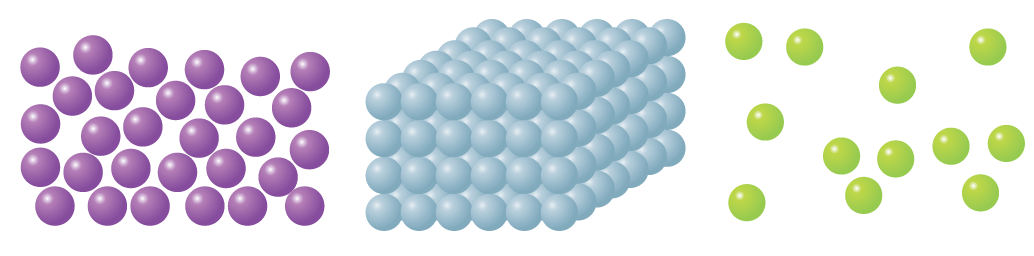
\includegraphics[scale=0.25]{Imagenes/Fisica_01.png}
     \end{figure}
     \begin{choices}
         \choice metal, gas, líquido.
         \choice solido, líquido, gas.
         \choice líquido, sólido, gas.
         \choice gel, gas, agua.
     \end{choices}
     \question ¿Cuánto es $\SI{10}{\kilo\meter\per\hour}$ en $\SI{}{\meter\per\second}$?
     \begin{choices}
        \choice $\SI{30.25}{\meter\per\second}$
        \choice $\SI{28.66}{\meter\per\second}$
        \choice $\SI{27.77}{\meter\per\second}$
        \choice $\SI{31.55}{\meter\per\second}$
    \end{choices}
    \question ¿Cuánto es $\SI{20}{\meter\per\second}$ en $\SI{}{\kilo\meter\per\minute}$?
     \begin{choices}
        \choice $\SI{1.2}{\kilo\meter\per\minute}$
        \choice $\SI{1.6}{\kilo\meter\per\minute}$
        \choice $\SI{1.8}{\kilo\meter\per\minute}$
        \choice $\SI{2.2}{\kilo\meter\per\minute}$
    \end{choices}
    \question Un venado se desplaza en una carretera recta con una velocidad de $\SI{72}{\kilo\meter\per\hour}$ durante $\SI{5}{\minute}$. ¿Qué distancia recorrió en ese tiempo?
    \begin{choices}
        \choice $\SI{4.75}{\kilo\meter}$
        \choice $\SI{5.95}{\kilo\meter}$
        \choice $\SI{6}{\kilo\meter}$
        \choice $\SI{8}{\kilo\meter}$
    \end{choices}
    \question ¿Cuáles son las propiedades físicas de los gases?
    \begin{choices}
        \choice Difusibilidad y volumen propio.
        \choice Volmen definido y maleabilidad.
        \choice Volumen y forma indefinida.
        \choice Forma indefinida y maleabilidad.
    \end{choices}
    \question La condensación del vapor de agua es un fenómeno físico por que:
    \begin{choices}
        \choice Solo se modifica la temperatura del agua.
        \choice Cambia la estructura del agua.
        \choice Cambia de estado físico.
        \choice Se altera la naturaleza propia del agua.
    \end{choices}
    \question Propiedad que nos permite cuantificar la cantidad de materiales de una mesa, una pelota, un cuaderno:
    \begin{choices}
        \choice Volumen.
        \choice Masa.
        \choice Longitud.
        \choice Densidad.
    \end{choices}
    \question Al cambio de estado de sólido a gas se le conoce como:
    \begin{choices}
        \choice Fusión.
        \choice Ebullición.
        \choice Sublimación.
        \choice Condensación.
    \end{choices}
    \question Un cohete despega por que empuja los gases de combustión con una fuerza $\mathbf{F}$ y éstos empujan al cohete con una fuerza:
    \begin{choices}
        \choice $\mathbf{F}$ nula y equilibrante.
        \choice $\mathbf{F}$ perpendicular y de sentido opuesto.
        \choice Del doble de $\mathbf{F}$ en sentido opuesto.
        \choice $\mathbf{F}$ en sentido opuesto.
    \end{choices}
    \question Cuando caminas sobre una alfombra y traes puestos tenis y ropa de nylon adquieres carga eléctrica, debida principalmente por:
    \begin{choices}
        \choice Frotamiento.
        \choice Conducción.
        \choice Inducción.
        \choice Contacto.
    \end{choices}
    \question La aguja de una brújula apunta siempre al norte por que:
    \begin{choices}
        \choice En el polo norto hay una mayor fuerza.
        \choice En el polo norte hay nua mayor cantidad de hierro.
        \choice En el polo norte el magnetismo es más intenso.
        \choice La aguja se alinea en la dirección del campo magnético de la Tierra.
    \end{choices}
    \question $\SI{50}{\degreeCelsius}$ es equivalente a
    \begin{choices}
        \choice $\SI{223}{\kelvin}$.
        \choice $\SI{64}{\degree} \, \text{F}$.
        \choice $\SI{323}{\kelvin}$.
        \choice $\SI{10}{\degree} \, \text{F}$.
        \choice $\SI{58}{\degree} \, \text{F}$.
    \end{choices}
    \question Al despejar $\mathbf{a}$ de la ecuación:
    \begingroup
    \abovedisplayskip=0pt
    \belowdisplayskip=-10pt
    \begin{align*}
   v_{f}^{2} = v_{i}^{2} + 2 \, a \, d
    \end{align*}
    \endgroup
    se obtiene:
    \begin{choices}
        \choice $a = v_{i}^{2} + 2 d v_{i}^{2}$
        \choice $a = \dfrac{v_{i}^{2} - v_{i}^{2}}{2 d}$
        \choice $a = \dfrac{v_{i}^{2} - v_{i}^{2}}{d}$
        \choice $a =v_{i}^{2} - 2 d v_{i}^{2}$
    \end{choices}


\section{Español.}

\subsection{Antónimos.}

De la siguiente lista de palabras, elige el correspondiente \textbf{antónimo}:
    \question Irrebatible:
    \begin{choices}
        \choice Discutible.
        \choice Triunfador.
        \choice Factible.
        \choice Inmemorable.
    \end{choices}
    \question Altruismo:
    \begin{choices}
        \choice Piedad.
        \choice Desinterés.
        \choice Benevolencia.
        \choice Egoísmo.
    \end{choices}
    \question Admisible:
    \begin{choices}
        \choice Prohibido.
        \choice Improbable.
        \choice Refutable.
        \choice Inaceptable.
    \end{choices}
    \question Tolerancia:
    \begin{choices}
        \choice Indulgencia.
        \choice Anuencia.
        \choice Tiranía.
        \choice Aguante.
    \end{choices}
    \question Postrar:
    \begin{choices}
        \choice Desanimar.
        \choice Vigorizar.
        \choice Desalentar.
        \choice Alegrar.
    \end{choices}
    \question Pertinaz:
    \begin{choices}
        \choice Constante.
        \choice Variable.
        \choice Continuo.
        \choice Duradero.
    \end{choices}
    \question Frenético:
    \begin{choices}
        \choice Errático.
        \choice Plácido.
        \choice Enojado.
        \choice Alegre.
    \end{choices}
    \question Fanatismo:
    \begin{choices}
        \choice Apatía.
        \choice Indeferencia.
        \choice Pereza.
        \choice Dejadez.
    \end{choices}
    \question Efímero:
    \begin{choices}
        \choice Inmortal.
        \choice Consante.
        \choice Inmutable.
        \choice Duradero.
    \end{choices}
    \question Arrebatar:
    \begin{choices}
        \choice Entregar.
        \choice Ceder.
        \choice Dar.
        \choice Congratular.
    \end{choices}

\subsection{Sinónimos.}

De las siguientes palabras, elige el correspondiente sinónimo.

    \question Flexible:
    \begin{choices}
        \choice Delgado.
        \choice Blando.
        \choice Liviano.
        \choice Elástico.
    \end{choices}
    \question Espacioso:
    \begin{choices}
        \choice Ancho.
        \choice Largo.
        \choice Extenso.
        \choice Bastante.
    \end{choices}
    \question Afable:
    \begin{choices}
        \choice Amable.
        \choice Ameno.
        \choice Gracioso.
        \choice Locuaz.
    \end{choices}
    \question Fino:
    \begin{choices}
        \choice Delicado.
        \choice Costoso.
        \choice Sútil.
        \choice Perfecto.
    \end{choices}
   \question Creyente:
    \begin{choices}
        \choice Verdadero.
        \choice Inteligente.
        \choice Místico.
        \choice Sabio.
    \end{choices}
    \question Egregio:
    \begin{choices}
        \choice Nombrado.
        \choice Conocido.
        \choice Célebre.
        \choice Solitario.
    \end{choices}
    \question Lucrativo:
    \begin{choices}
        \choice Ruidoso.
        \choice Fructífero.
        \choice Orgulloso.
        \choice Benéfico.
    \end{choices}
    \question Lugar:
    \begin{choices}
        \choice Región.
        \choice Paraje.
        \choice Sitio.
        \choice Mapa.
    \end{choices}
    \question Extraño:
    \begin{choices}
        \choice Diferente.
        \choice Preclaro.
        \choice Exótico.
        \choice Excelente.
    \end{choices}
    \question Superficial:
    \begin{choices}
        \choice Tranparente.
        \choice Banal.
        \choice Externo.
        \choice Interno.
    \end{choices}
\end{questions}
\end{multicols}
\end{document}